\documentclass[a4paper,10pt]{article}
\usepackage[utf8]{inputenc}
\usepackage[T1]{fontenc}	
\usepackage[italian]{babel}

\usepackage{amsmath}
\usepackage{amsfonts}
\usepackage{amssymb}
\usepackage{graphicx}

\usepackage[left=2cm,right=2cm,top=2cm,bottom=2cm]{geometry}
\geometry{a4paper}

\usepackage{booktabs}
\usepackage{verbatim}
\usepackage{subfig}

\usepackage[cdot, thickqspace, squaren]{SIunits}
\usepackage{float}
% macro
\def\code#1{\texttt{#1}}

\title{Esperienza di Ottica 1}
\author{Gruppo BL \\ Candido Alessandro, Luzio Andrea, Mazziotti Fabrizio}

\begin{document}

\maketitle

\section{Scopo}
L'esperienza è divisa in due parti:
\begin{itemize}
	\item nella prima parte si vuole determinare la lunghezza d’onda di una riga spettrale emessa dal sodio (la riga gialla);
	\item nella seconda parte ci sono due obiettivi:
	\begin{itemize}
		\item il primo è di valutare la risoluzione dello strumento di misura, uno spettroscopio a reticolo, nella misura delle linee emesse da lampade spettrali;
		\item il secondo è quello di determinare la costante di Rydberg dalla misura della lunghezza d’onda delle righe di emissione dell’idrogeno.
	\end{itemize}
\end{itemize}

\section{Esperienza A: Misura della lunghezza d'onda della riga gialla del sodio}

\subsection{Strumentazione}

\begin{itemize}
	\item spettroscopio a prisma:
	\begin{itemize} %questa lista è solo un abbozzo, devo scriverla bene
		\item due telescopi;
		\item prisma con supporto;
		\item struttura di base, con possibilità di ruotare il supporto del prisma e blocco per la posizione, e possibilità di ruotare il telescopio d'osservazione, con blocco e goniometro dotato di nonio per la misura della posizione del telescopio stesso.
	\end{itemize}
	\item lampada al cadmio;
	\item lampada al sodio;
	\item lente d'ingrandimento, per la lettura del nonio;
	\item torcia.
\end{itemize}

\begin{figure}[H]
	\centering
	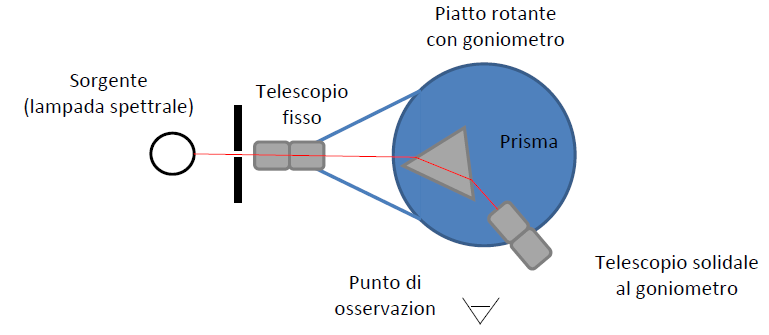
\includegraphics[width=0.7\textwidth]{../grafici/Schema1.png}
	\caption{Schema dell'apparato usato}
	\label{fig:schema1}
\end{figure}

\subsection{Calibrazione dello strumento con la lampada al cadmio}

Si è accesa la lampada al cadmio e dopo aver atteso qualche minuto, per far sì che andasse in temperatura, si sono eseguite le seguenti operazioni.

\paragraph{Determinazione dello "zero" del goniometro} Come prima cosa si è rimossa la torretta e si è posizionata approssimativamente la lampada in modo che la fessura raccogliesse più luce possibile. 

Si è dunque allineato il telescopio di osservazione e si è migliorato il posizioamento della lampada, decidendo assieme l'apertura della slitta d'ingresso. Per fare ciò si è riposizionato anche il prisma per verificare l'effetto dell'apertura della slitta sulla visualizzazione delle righe spettrali; un'apertura troppo ristretta non consentiva il passaggio di abbastanza luce, viceversa se troppo larga si aveva ambiguità sulla posizione della riga e, decisamente più importante, la luce delle righe più intense diventa troppa, al punto da peggiorare la visualizzazione di quelle meno intense.

Si è infine acquisito l'angolo ($\alpha_0$) a cui veniva osservata la luce non deflessa, a partire dall'uscita del telescopio fisso. Come indicato la misura è stata effettuata da tutti i componenti del gruppo, ottenendo così 3 misure, al fine di valutare l'errore sistematico associato al metodo di misura.
Si è trovato: $\alpha_0 = 10\degree~53'~42''\pm 1'~32''$
% la notazione in gradi è doppiamente posizionale, quindi non so bene come regolarmi con le cifre significative, ho messo i decimali giusti, ma converiti in secondi sembrano un obbrobrio

\begin{table}[H]
	\centering
	\begin{tabular}{c|c|c}
		$10\degree~55'$  & $10\degree~52'$ & $10\degree~54'$\\
	\end{tabular}
\caption{Dati raccolti sulla misura di $\alpha_0$}
\end{table}

Si è inoltre stimato indipendentemente che, data la larghezza dell'oculare, il singolo osservatore poteva compiere un errore massimo di parallasse pari a circa $2\degree-3\degree$ complessivi (ampiezza dell'intervallo), quindi circa $\pm 1\degree-1.5\degree$, si è in seguito supposto che fosse già incluso nelle fluttuazioni considerate con la misura da parte di più osservatori.

\paragraph{Determinazione della condizione di minima deviazione} Si è osservato lo spostamento dell righe spettrali del cadmio in funzione della posizione del prisma, e si è individuata la posizione corrispondente alla condizione di minimo spostamento relativa alla riga verde, la più vicina alla riga gialla attesa del sodio.

Si è notato che la posizione della riga verde era stazionaria, entro la sensibilità consentita dall'apparato, per un certo intervallo di posizioni del prisma, si è perciò sfruttata questa indeterminazione (più correttamente: si è cercato di ridurla) imponendo approssimativamente la condizione di minimo spostamento anche per la riga rossa.
L'inesattezza in quest'ultima operazione è introdotta dal fatto che fosse difficile per l'osservatore assicurare che la condizione, che veniva verificata dinamicamente ruotando il prisma, fosse rispettata da entrambe le righe; si è dunque privilegiato la riga verde, in quanto era stata individuata in principio come la più vicina alla zona d'interesse.

Il prisma è stato dunque bloccato nella posizione individuata, e non è stato più mosso nel seguito dell'esperienza A.

\paragraph{Calibrazione della scala spettrale} 

Si sono misurate le posizioni delle righe del cadmio nel modo descritto per l'individuazione dello zero. I valori di tutte le misure sono riportati in \tablename{~\ref{tab:cadmio}.

\begin{table}[H]
	\centering
	\begin{tabular}{c|c|c|c}
	blu & azzurro & verde & rosso \\
	\hline
	$60\degree~39'$ & $60\degree~29'$ & $60\degree~0'$ & $58\degree~43'$\\
	$60\degree~40'$ & $60\degree~26'$ & $60\degree~0'$ & $58\degree~41'$\\
	$60\degree~41'$ & $60\degree~28'$ & $60\degree~0'$ & $58\degree~44'$\\
	\end{tabular}
	\caption{Misura delle righe del cadmio}
	\label{tab:cadmio}
\end{table}

Si è quindi eseguito un fit affine per la calibrazione della scala spettrale, si riporta il grafico in \figurename{~\ref{fig:cadmio}.

\begin{figure}[H]
	\centering
	\includegraphics[width=0.7\textwidth]{../grafici/calcadmio.pdf}
	\caption{Dati sperimentali e fit affine delle righe spettrali del cadmio}
	\label{fig:cadmio}
\end{figure}

I risultati ottenuti dal fit per coefficiente angolare ($m$) ed intercetta ($q$) sono riportati di seguito in \tablename{~\ref{tab:calcadmio}.
	

\begin{table}[H]
	\centering
	\begin{tabular}{c|c}
		$m$ & $\unit{0.373 \pm 0.009}{eV/~\degree}$ \\
		\hline
		$q$ & $\unit{-15.9 \pm 0.4}{eV}$ \\
	\end{tabular}
	\caption{Parametri ottenuti dal fit}
	\label{tab:calcadmio}
\end{table}

\subparagraph{Riga viola} Si è inoltre misurata un ulteriore riga nella regione viola dello spettro, l'intensità di questa riga era però molto debole, la misura è stata quindi notevolmente meno precisa.
Si riportano i dati raccolti in \tablename{~\ref{tab:viola}.
	
\begin{table}[H]
	\centering
	\begin{tabular}{c|c|c}
		$61\degree~15'$  & $61\degree~16'$ & $61\degree~11'$\\
	\end{tabular}
	\caption{Dati raccolti sulla riga viola}
	\label{tab:viola}
\end{table}
	
Non si è incluso questo valore nel fit perché non era a disposizione un valore corrispondente della lunghezza d'onda con cui confrontarlo.
% ce lo scrivo questo?

\subsection{Misura della lunghezza d’onda della riga osservata del sodio}

\paragraph{Riga di emissione gialla}
Si è misurata la riga di emissione del sodio nella regione gialla dello spettro, con la stessa modalità adottata per le righe del cadmio.
Si riportano le misure in \tablename{~\ref{tab:gialloNa}.

\begin{table}[H]
	\centering
	\begin{tabular}{c|c|c}
		$61\degree~15'$  & $61\degree~16'$ & $61\degree~11'$\\
	\end{tabular}
	\caption{Dati raccolti sulla riga viola}
	\label{tab:gialloNa}
\end{table}

Dalla calibrazione effettuata con il cadmio si ottiene che la lunghezza d'onda corrispondente alla riga è: $\lambda_{yellow, Na} = \unit{594 \pm 6}{\nano\meter}$, cioè ha un'energia pari a $E_{yellow, Na} = \unit{2.086\pm0.020}{e\volt}$.

\paragraph{Altre righe}

Si sono misurate anche altre righe del sodio, si riportano in \tablename{~\ref{tab:moreNa} i vari valori e le relative lunghezze d'onda associate.

\begin{table}[H]
	\centering
	\begin{tabular}{c|c|c|c|c|c}
		colore &	&	&	& misura & lunghezza d'onda [nm]\\
		\hline
		rosso &	$58\degree~55'$ & $58\degree~53'$ & $58\degree~56'$ & $58\degree~54'~40'' \pm 1'~30''$ & $618 \pm 5$\\
		verde & $59\degree~18'$ & $59\degree~20'$ & $59\degree~16'$ & $59\degree~18' \pm 2'$  & $576 \pm 5$\\
		verde scuro & $59\degree~55'$ & $59\degree~55'$ & $59\degree~55'$ & $59\degree~55' \pm 1'$ & $520 \pm 9$\\
		azzurro & $60\degree~8'$ & $60\degree~10'$ & $60\degree~6'$ & $60\degree~8' \pm 2'$& $503 \pm 4$\\
		viola & $60\degree~39'$ & $60\degree~39'$ & $60\degree~39'$ & $60\degree~39' \pm 1'$ & $467 \pm 7$\\	
	\end{tabular}
	\caption{Misura delle ulteriori righe del sodio}
	\label{tab:moreNa}
\end{table}

L'intensità delle altre righe era per tutte minore rispetto a quella della riga gialla, ma alcuna eran comunque ben visibili, mentre, anche in questo caso, la riga nella regione viola dello spettro lo era poco.

Si è provato a migliorare la visualizzazione della riga viola muovendo la slitta d'ingresso, ottenendo però modesti risultati.

\section{Esperienza B: Misura della costante di Rydberg}

\subsection{Strumentazione}

\begin{itemize}
	\item spettroscopio a reticolo di diffrazione:
%stesse cose di sopra da aggiungere

	\item lampada al mercurio;
	\item lampada al idrogeno;
	\item lampada al sodio;
	\item lente d'ingrandimento, per la lettura del nonio;
	\item torcia.
\end{itemize}

\begin{figure}[H]
	\centering
	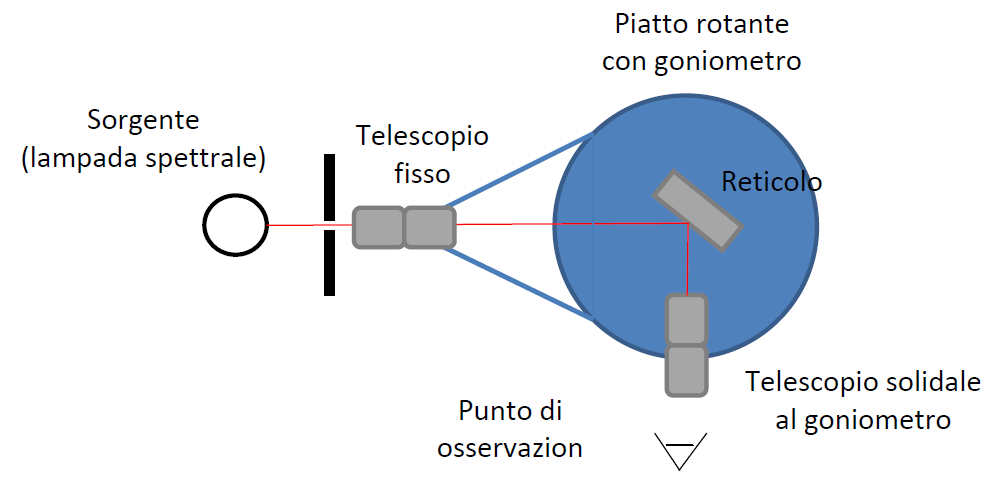
\includegraphics[width=0.7\textwidth]{../grafici/Schema2.png}
	\caption{Schema dell'apparato usato}
	\label{fig:schema2}
\end{figure}

\subsection{Regolazione della geometria dei telescopi}
Lo schema dell'apparato è rappresentato in figura \figurename{~\ref{fig:reticolo}}.

In primo luogo si è posizionata la lampada al mercurio vicino al telescopio fisso e si è ruotato il telescopio di osservazione fino ad osservare l'ordine zero di diffrazione. Si è fissato questo telescopio e si è regolato lo spessore della fenditura, la distanza della lampada da essa e la messa a fuoco del telescopio per visualizzare la riga con la maggior intensità possibile e con uno spessore né troppo piccolo da non permettere la visualizzazione della riga, né troppo grande per evitare di avere un'incertezza grande sulla effettiva posizione della riga rispetto alle distanze in gioco\footnote{La distanza tra i due bordi della riga dell'ordine zero (e poi anche di quelle di ordine superiore), nelle condizioni scelte nell'esperienza, è stimata essere minore di ???(io direi 0.5') che è da confrontare con la scala graduata del nonio, la cui risoluzione massima è di 0.5'.}.
%da completare
La distanza della lampada dalla fenditura non deve essere né troppo grande ($\sim 1 cm$) perché ne risentirebbe la luminosità delle riga, né troppo piccola perché si vedrebbero aloni intorno ad essa.
Si sono poi osservate le righe del primo ordine di diffrazione (quelle più intense,cioè, in ordine per angolo di incidenza decrescente: viola, verde, rosso e un doppietto giallo) e si è verificato che, con gli stessi accorgimenti fatti per la riga dell'ordine zero, esse siano ben messe a fuoco.

\subsection{Calibrazione dello strumento e misura del passo reticolare}
Con la stessa procedura effettuata nella parte A si è effettuata la calibrazione del nonio ottenendo $\alpha_0 = $\footnote{La trattazione dei vari dati acquisiti in questa parte dell'esperienza e dei relativi errori sono trattati nell'apposita sezione 'errori sistematici'.}. Presa questa misura, tutte le letture successive fatte sul nonio e riportate qui saranno riferite a questo valore.

\begin{figure}[H]
	\centering
	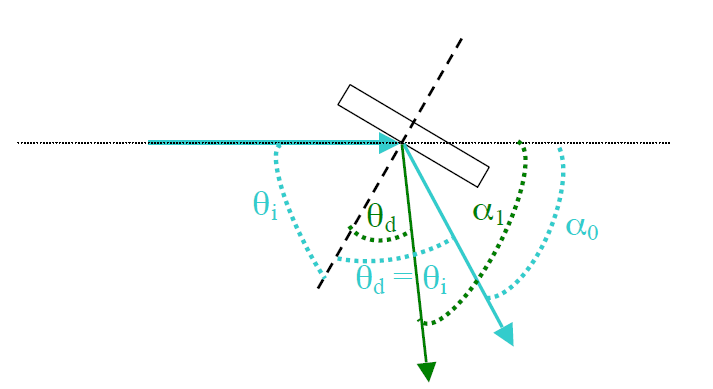
\includegraphics[width=0.7\textwidth]{../grafici/Angoli.png}
	\caption{Schema dell'apparato usato}
	\label{fig:angoli}
\end{figure}

\paragraph{Misura del passo reticolare}
Si Il passo reticolare è stato misurato conoscendo la lunghezza d'onda della riga verde del sodio. Sono stati misurati, relativi all'angolo di calibrazione $\theta_0 =348\degree 42' \pm  2' $, l'angolo della riflessione speculare $8\degree 55.7' \pm 0.5'$ e del primo massimo di interferenza della riga verde del mercurio $69\degree 29.0'\pm 1'$. Nota la lunghezza d'onda della suddetta linea $546.074 \pm 0.001 nm$ si è usata la nota equazione $d(sin \theta_i– sin \theta_d) = m\lambda$ per stimare il passo reticolare $d$. Gli errori sono stati propagati tenendo conto delle covarianze e i dati presi sono stati considerati con errori statistici\footnote{Si è ritenuto possibile considerare gli errori come statistici in quanto frutto della media di dati presi da persone diverse. Fra le prese dati dei vari elementi del gruppo si ha avuto cura di riportare il telescopio di osservazione in una zona neutra, in modo di evitare eventuali influenze da parte di membri del gruppo su altri} e scorrelati.


Il risultato ottenuto è dunque $d=835.57 \pm 0.25 nm$ (ovvero $1196.8+/-0.4$ linee per mm). Il risultato sembra compatibile con quanto atteso.

\subsection{Righe di emissione dell'idrogeno}
Per misurare la lunghezza d'onda delle linee dell'idrogeno si è deciso di diminuire l'angolo di incidenza del fascio entrante sul reticolo. Questo \footnote{Secondo il gruppo e parte dei membri dello staff del lab, fra questi c'è molta confusione a riguardo} dovrebbe aumentare la potenza delle righe osservate. Si è misurato un angolo di deviazione in riflessione di $46\degree 3' \pm 2'$. Riferiti a tale angolo sono stati misurati i seguenti dati.

\begin{table}[H]
	\centering
	\begin{tabular}{c|c|c|c|c|c|c|c}
		colore & $\alpha_i$ &	$\theta_i$ & ordine & lunghezza d'onda [nm] & attesa[nm]& $n_2$ (serie) & $n_1$\\
		\hline
azzurro &  $ 93\degree 7.0' \pm 2.0 ' $  &  $ 19\degree 54.0' \pm 2.0 ' $  &  $ 1 $ & $ 484.5+/-0.6 $ & $ 0 $ & $ 2 $ \\
rosso &  $ 105\degree 16.0' \pm 2.0 ' $  &  $ 7\degree 45.0' \pm 2.0 ' $  &  $ 1 $ & $ 656.3+/-0.6 $ & $ 0 $ & $ 2 $ \\
azzurro &  $ 127\degree 13.0' \pm 2.0 ' $  &  $ -15\degree 48.0' \pm 2.0 ' $  &  $ 2 $ & $ 486.93+/-0.32 $ & $ 0 $ & $ 2 $ \\
d-viola &  $ 83\degree 7.0' \pm 2.0 ' $  &  $ 29\degree 54.0' \pm 2.0 ' $  &  $ 1 $ & $ 352.4+/-0.5 $ & $ 0 $ & $ 1 $ \\
d-verde &  $ 96\degree 18.0' \pm 3.0 ' $  &  $ 16\degree 43.0' \pm 3.0 ' $  &  $ 1 $ & $ 528.5+/-0.8 $ & $ 0 $ & $ 2 $ \\
rosso &  $ 102\degree 29.0' \pm 2.0 ' $  &  $ 10\degree 32.0' \pm 2.0 ' $  &  $ 1 $ & $ 616.1+/-0.6 $ & $ 0 $ & $ 2 $ \\
viola &  $ 119\degree 18.0' \pm 3.0 ' $  &  $ -7\degree 43.0' \pm 3.0 ' $  &  $ 2 $ & $ 430.2+/-0.4 $ & $ 0 $ & $ 2 $ \\
	\end{tabular}
	\caption{Misura delle righe spettrali dell'idrogeno, la d nel nome significa che in realtà la linea è un doppietto, di cui un componente è talmente fioco da non essere stato misurabile. Si noti come il primo azzurro e il secondo dovrebbero essere la stessa linea spettrale viste al primo e al secondo massimo di interferenza. I valori sono simili MA NON PIENAMENTE COMPATIBILI, PERCH\'E ????
I valori di $n_1$ e $n_2$ sono quelli che compaiono nell'equazione $1/\lambda=Ry(1/n_1^2-1/n_2^2)$. La serie Balmer corrisponde a $n_2=2$. $n_2=1$ è la serie Lyman.	
	}
	\label{tab:HH}
\end{table}
La stima dei numeri quantici coinvolti è stata fatta con la misura di riferimento del $Ry=1.097373156 * 10^{-2} nm^{-1}$\footnote{ Questo valore è privo della correzione apportata dalla massa finita del nucleo dell'ordine del 1 per mille).(che schifo, la nota si mescola con l'esponente...)} . Questo processo è stato svolto essenzialmente a mano...

 

\subsection{Misura del doppietto del sodio}



%io metterei qui tutta la spiegazione del fatto che abbiamo fatto ciascuno la nostra misura ecc in modo da mettere in tutte le altre parti solo il risultato finale.
\subsection{Errori sistematici}

\end{document}